\documentclass{article}


% if you need to pass options to natbib, use, e.g.:
%     \PassOptionsToPackage{numbers, compress}{natbib}
% before loading neurips_2022


% ready for submission
\usepackage[preprint,nonatbib]{neurips_2022}


% to compile a preprint version, e.g., for submission to arXiv, add add the
% [preprint] option:
%     \usepackage[preprint]{neurips_2022}


% to compile a camera-ready version, add the [final] option, e.g.:
%     \usepackage[final]{neurips_2022}


% to avoid loading the natbib package, add option nonatbib:
%    \usepackage[nonatbib]{neurips_2022}


\usepackage[utf8]{inputenc} % allow utf-8 input
\usepackage[T1]{fontenc}    % use 8-bit T1 fonts
\usepackage{hyperref}       % hyperlinks
\usepackage{url}            % simple URL typesetting
\usepackage{booktabs}       % professional-quality tables
\usepackage{amsfonts}       % blackboard math symbols
\usepackage{amsmath}
\usepackage{amsthm}
\usepackage{nicefrac}       % compact symbols for 1/2, etc.
\usepackage{microtype}      % microtypography
\usepackage{xcolor}         % colors
\usepackage[backend=biber]{biblatex}
\usepackage{graphicx}
\usepackage{subcaption}

\newtheorem{assumption}{Assumption}
\newtheorem{definition}{Definition}
\newtheorem{theorem}{Theorem}

\addbibresource{reference.bib}


\title{Formatting Instructions For NeurIPS 2022}


% The \author macro works with any number of authors. There are two commands
% used to separate the names and addresses of multiple authors: \And and \AND.
%
% Using \And between authors leaves it to LaTeX to determine where to break the
% lines. Using \AND forces a line break at that point. So, if LaTeX puts 3 of 4
% authors names on the first line, and the last on the second line, try using
% \AND instead of \And before the third author name.


\author{%
  Xiaoxuan Yu \\
  College of Chemistry and Molecular Engineering\\
  Peking University\\
  Beijing, China \\
  \texttt{xiaoxuan\_yu@pku.edu.cn} \\
  % examples of more authors
  \And
  Yihang Xia \\
  School of Mathematical Sciences \\
  Peking University \\
  Beijing, China\\
  \texttt{xyh-mathematics@pku.edu.cn} \\
  % \AND
  % Coauthor \\
  % Affiliation \\
  % Address \\
  % \texttt{email} \\
  % \And
  % Coauthor \\
  % Affiliation \\
  % Address \\
  % \texttt{email} \\
  % \And
  % Coauthor \\
  % Affiliation \\
  % Address \\
  % \texttt{email} \\
}


\begin{document}


\maketitle


\begin{abstract}
  The abstract paragraph should be indented \nicefrac{1}{2}~inch (3~picas) on
  both the left- and right-hand margins. Use 10~point type, with a vertical
  spacing (leading) of 11~points.  The word \textbf{Abstract} must be centered,
  bold, and in point size 12. Two line spaces precede the abstract. The abstract
  must be limited to one paragraph.
\end{abstract}


%\section{Overview}
%\label{overview}

\section{Problem setup and backgrounds}

The article studies gradient-based optimization methods obtained by directly
discretizinga second-order ordinary differential equation (ODE) related to the
continuous limit of Nesterov's accelerated gradient method. It introduces some
conditions under which the sequence of iterates generated by discretizing the
proposed second-order ODE converges to the optimal solution at a certain rate.\\\\
Firstly let's focus the essential target problem:
\begin{align}\label{min}
  \mathop{\mathrm{min}}\limits_{x \in \mathbb{R}^{d}} f(x),
\end{align}
where $f$ is convex and sufficiently smooth. For solving \ref{min}, there are several
methods.
\begin{itemize}
  \item Classical method: gradient decent, which displays a sub-optimal convergence rate of $\mathcal{O}(N^{-1})$.
  \item Nesterov's seminal accelerated gradient method, matches the oracle lower bound of $\mathcal{O}(N^{-2})$.
\end{itemize}
Several articles have pursued approaches to \textsc{Nag} (and accelerated methods in general)
via a continuous-time perspective. However, they fail to provide a general
discretization procedure that generates provably convergent accelerated methods.
This article takes Runge-Kutta integrater as tool and introduces a second-order ODE
that generates an accelerated first-order method for smooth functions if using
Runge-Kutta method.\\\\
\textcolor{red}{Place for introduction to additional related work if necessary.}

\section{Main results}
To build up a iterative method, letting $x_{0}$ be the initial point, firstly we
consider the sublevel set
\begin{align}\label{sublevel_set}
  \mathcal{S} := \{ x \in \mathbb{R}^{d} | f(x) \leq \mathrm{exp}(1) (f(x_{0})
  - f(x^{*}) + \|x_{0} - x^{*}\|^{2}) + 1 \},
\end{align}
where $x^{*}$ is the minimum of \ref{min}. The introduction of set $\mathcal{S}$
actually gives a restriction of the sequence of iterates obtained from
discretizing a suitable ODE (would be proved later). Denote subset
\begin{align}
  \mathcal{A} := \{ x \in \mathbb{R}^{d} | \exists x' \in \mathcal{S}, \|x-x'\| \leq 1 \},
\end{align}
Then all assumptions we may require can be considered just in $\mathcal{A}$.

\begin{assumption}
  There exists an integer $p \geq 2$ and a positive constant L such that for any point $x \in \mathcal{A}$, and for all indices $i \in \{1,\ldots,p-1\}$, we have the lower-bound
  \begin{align}\label{assum_1}
    f(x) - f(x^{*}) \geq \frac{1}{L} \| \nabla^{(i)}f(x) \|^{\frac{p}{p-i}},
  \end{align}
  where $x^{*}$ minimizes f and $\| \nabla^{(i)}f(x) \|$ denotes the operator norm of the tensor $\nabla^{(i)}f(x)$.
\end{assumption}

\begin{assumption}
  There exists an integer $s \geq p$ and a constant $M \geq 0$, such that $f(x)$ is order $(s+2)$ differentiable. Furthermore, for any $x \in \mathcal{A}$, the following operator norm bounds hold:
  \begin{align}\label{assum_2}
    \| \nabla^{(i)}f(x) \| \leq M,\ \text{for}\ i = p,p+1,\ldots,s,s+1,s+2.
  \end{align}
\end{assumption}

When the sublevel sets of $f$ are compact and hence the set $\mathcal{A}$ is also compact; as a result, the bound \ref{assum_2} on high order derivatives is implied by continuity.

\subsection{Runge-Kutta\ integrators}

The explicit Runge-Kutta integrators used in the article appears in the form below.

\begin{definition}
  Given a dynamical system $\dot{y} = F(y)$, let the current point be $y_{0}$ and the step size be $h$. An explicit $S$ stage Runge-Kutta method generates the next step via the following update:
  \begin{align}\label{def_1}
    g_{i} = y_{0} + h \sum\limits_{j=1}^{i-1} a_{ij}F(g_{j}),\ \ \ \Phi_{h}(y_{0}) = y_{0}
    + h \sum\limits_{i=1}^{S} b_{i}F(g_{i}),
  \end{align}
  where $a_{ij}$ and $b_{i}$ are suitable coefficients defined by the integrator; $\Phi_{h}(y_{0})$ is the estimation of the state after time step $h$, while $g_i$ (for $i = 1,\ldots,S$) are a few neighboring points where the gradient information $F(g_i)$ is evaluated.
\end{definition}

In general, Runge-Kutta methods offer a powerful class of numerical integrators, and with the knowledge
of its concergence behaviour when discretizing for solutions, the article gets to use it
to discretize ODE with controlment of its convergence rates.

\subsection{Formal work and inspiration}

Then focus on the \textsc{Nag} method that is defined according to the updates
\begin{align}\label{nag}
  x_{k} = y_{k-1} - h \nabla f(y_{k-1}),\ \ \ y_{k} = x_{k} + \frac{k-1}{k+2} (x_{k} - x_{k-1}).
\end{align}
\textcite{JMLR:v17:15-084} showed that the iteration \ref{nag} in the limit is equivalent to the
following ODE
\begin{align}\label{nag_ode_1}
  \ddot{x}(t) + \frac{3}{t} \dot{x}(t) + \nabla f(x(t)) = 0,\ \ \ \mathrm{where\ }
  \dot{x} = \frac{dx}{dt}
\end{align}
when one drives the step size $h$ to zero. It can be further shown that in the
continuous domain the function value $f(x(t))$ decreases at the rate of $\mathcal{O}(1/t2)$
along the trajectories of the ODE. This convergence rate can be accelerated to an
arbitrary rate in continuous time via time dilation as in [Wibisono et al., 2016].
In particular, the solution to
\begin{align}\label{nag_ode_2}
  \ddot{x}(t) + \frac{p+1}{t} \dot{x}(t) + p^{2}t^{p-2} \nabla f(x(t)) = 0
\end{align}
has a convergence rate $\mathcal{O}(1/t^{p})$. When $p > 2$, Wibisono et al. [2016] proposed rate matching
algorithms via utilizing higher order derivatives. However, this article focuses purely on
first-order methods and study the stability of discretizing the ODE directly when
$p \geq 2$.
\\\\According to some related work, deriving the ODE from the algorithm is now a solved
problem. Nevertheless, to derive the update of \textsc{Nag} or any other
accelerated method by directly discretizing an ODE is not. Some work points out that
explicit Euler discretization of the ODE in \ref{nag_ode_1} may not lead to a stable
algorithm. \textcite{https://doi.org/10.48550/arxiv.1802.03653} observed empirically that Verlet
integration is stable and suggested that the stability relates to the symplectic
property of the Verlet integration, but for dissipative systems such as \ref{nag_ode_2},
this doesn't hold. This article offers a different approach: it augments the state with
time in \ref{nag_ode_2}, and focuses the following ODE
\begin{align}\label{nag_ode_final}
  \ddot{x}(t) + \frac{2p+1}{t} \dot{x}(t) + p^{2}t^{p-2} \nabla f(x(t)) = 0.
\end{align}
This actually turns the non-autonomous dynamical system into an autonomous one.

\subsection{Main\ conclusion}

The ODE in \ref{nag_ode_final} can also be written as the dynamical system
\begin{align}\label{equation}
  \dot{y} = F(y) = \begin{bmatrix}
                     -\frac{2p+1}{t} v - p^{2}t^{p-2} \nabla f(x) \\
                     v                                            \\
                     1
                   \end{bmatrix},\ \ \ \mathrm{where\ }y = [v;x;t].
\end{align}
\textbf{Algorithm\ 1:\ }Input$(f,x_{0},p,L,M,s,N)$ \hfill $\triangleright$ Constants
$p,L,M$ are the same as in Assumptions\\
1. Set the initial state $y_{0} = [\overrightarrow{0};x_{0};1] \in \mathbb{R}^{2d+1}$\\
2. Set step size $h = C/N^{(1/s+1)}$ \hfill $\triangleright$ C is determined by
$p,L,M,s,x_{0}$\\
3. $x_{N} \leftarrow $ Oreder-s-Runge-Kutta-Integrater($F,y_{0},N,h$) \hfill $\triangleright$
F is defined in equation \ref{equation}\\
4. \textbf{return} $x_{N}$\\\\
Since the article has augmented the state with time to obtain an autonomous system,
it can be readily solved numerically with a Runge-Kutta integrator as in
\textbf{Algorithm 1}.

\begin{theorem}
  Consider the second-order ODE in \ref{nag_ode_final}. Suppose that the function $f$ is convex and Assumptions 1 and 2 are satisfied. Further, let s be the order of the Runge-Kutta integrator used in \textbf{Algorithm 1}, $N$ be the total number of iterations, and $x_0$ be the initial point. Also, let $\mathcal{E}_{0} := f(x_{0}) - f(x^{*}) + \|x_{0} - x^{*}\|^{2} + 1$. Then, there exists a constant $C_1$ such that if we set the step size as $h = C_{1}N^{-1/(s+1)} (L+M+1)^{-1}\mathcal{E}_{0}^{-1}$, the iterate $x_N$ generated after running \textbf{Algorithm 1} for N iterations satisfies the inequality
  \begin{align}\label{thereom_1}
    f(x_{N}) - f(x^{*}) \leq C_{2}\mathcal{E}_{0} \left[
      \frac{(L+M+1)\mathcal{E}_{0}}{N^{\frac{s}{s+1}}} \right]^{p} = \mathcal{O}
    (N^{-p\frac{s}{s+1}}),
  \end{align}
  where the constants C1 and C2 only depend on $s, p$, and the Runge-Kutta integrator. Since each iteration consumes S gradient, $f(x_N) - f(x^{*})$ will converge as $\mathcal{O}(S^{\frac{ps}{s+1}}N^{-\frac{ps}{s+1}})$ with respect to the number of gradient evaluations. Note that for commonly used Runge-Kutta integrators, $S \leq 8$.
\end{theorem}
% \subsubsection*{Application to logistic loss}
\section{Numerical Experiments}
In this section, we implement the algorithms in the original article with \texttt{Julia} and its package \texttt{DifferentialEquations.jl} \cite{rackauckas2017differentialequations}. By comparing ODE direct discretizating (DD) methods described in the article against gradient descent (GD) and Nesterov's accelerated gradient (NAG) methods, we can verify the main results in the theoretical part. The code of these experiments can be found here: \url{https://github.com/xiaoxuan-yu/Direct-Runge-Kutta-Discretization-Achieves-Acceleration-PKU}.

Inspired by the numerical results by \textcite{NEURIPS2019_7a2b33c6}, we generate normal distributed separable dataset and fit a linear model \(Ax=b\). Then, we minimize three different kinds of loss functions:
\begin{equation}
    \begin{aligned}
        f_1(x) & = \left\| Ax-b \right\|_{2}^2                \\
        f_2(x) & = \sum_{i}\log(1+e^{-w_i^{\mathrm{T}}x y_i}) \\
        f_3(x) & = \frac{1}{4}\left\| Ax-b \right\|_{4}^4
    \end{aligned}
\end{equation}
where $f_1(\cdot ),f_2(\cdot ),f_3(\cdot )$ are $L_2$ loss, logistic loss and $L_4$ loss, respectively. For each test case and optimization algorithm, we empirically select the learning rate as the largest step length among $\{ 10^{-k}|k\in \mathbb{Z} \}$ that the method remains stable during the optimization process. Main results are shown in Figure \ref{Numerical} where all figures are on log-log scale.
\begin{figure}[htbp]
    \begin{subfigure}{0.45\textwidth}
        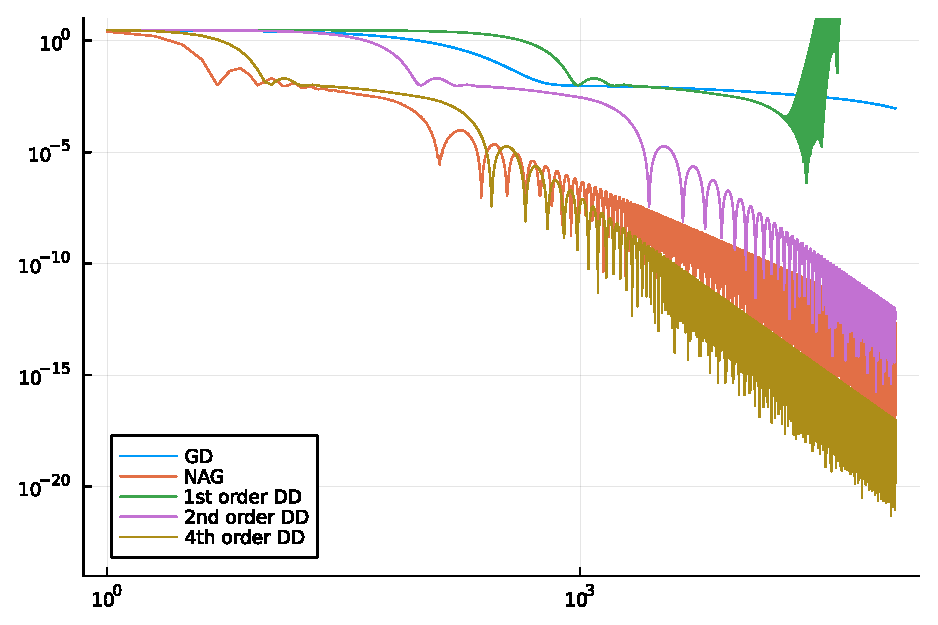
\includegraphics[width=\textwidth]{"assets/quadratic-1.pdf"}
        \caption{}
        \label{fig:l2-1}
    \end{subfigure}
    \hfill
    \begin{subfigure}{0.45\textwidth}
        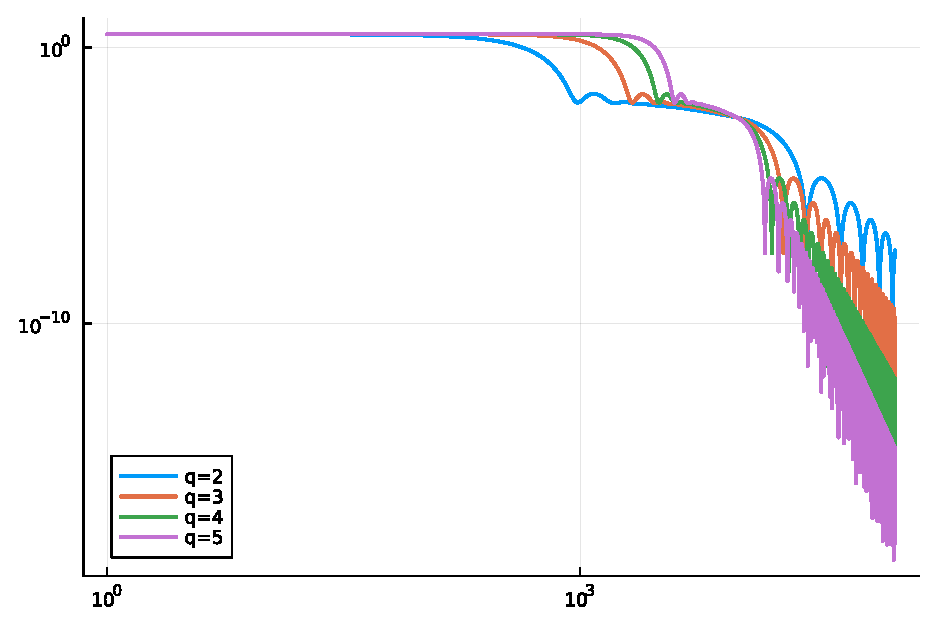
\includegraphics[width=\textwidth]{"assets/quadratic-2.pdf"}
        \caption{}
        \label{fig:l2-2}
    \end{subfigure}
    \hfill
    \begin{subfigure}{0.45\textwidth}
        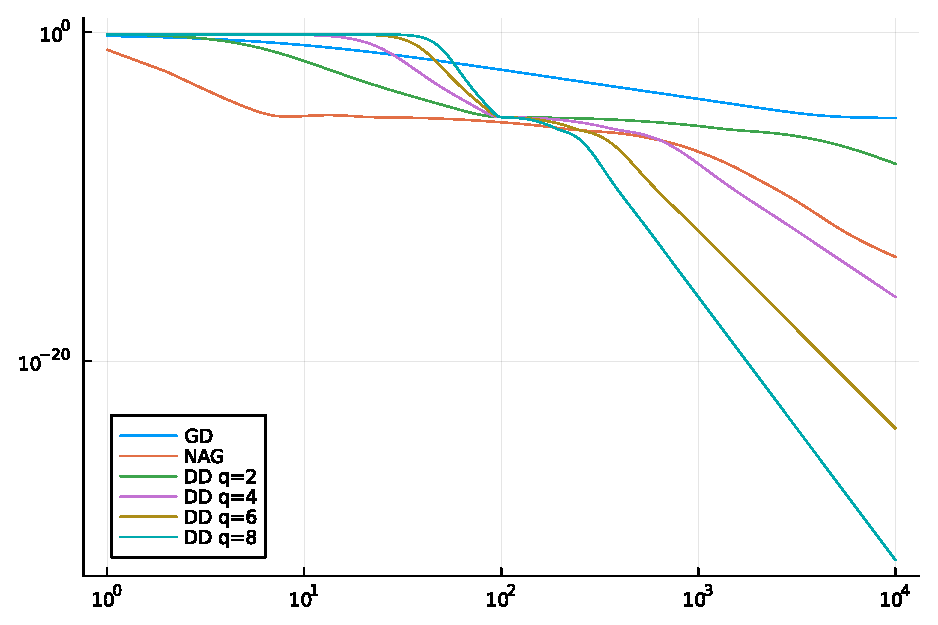
\includegraphics[width=\textwidth]{"assets/l4loss.pdf"}
        \caption{}
        \label{l4}
    \end{subfigure}
    \hfill
    \begin{subfigure}{0.45\textwidth}
        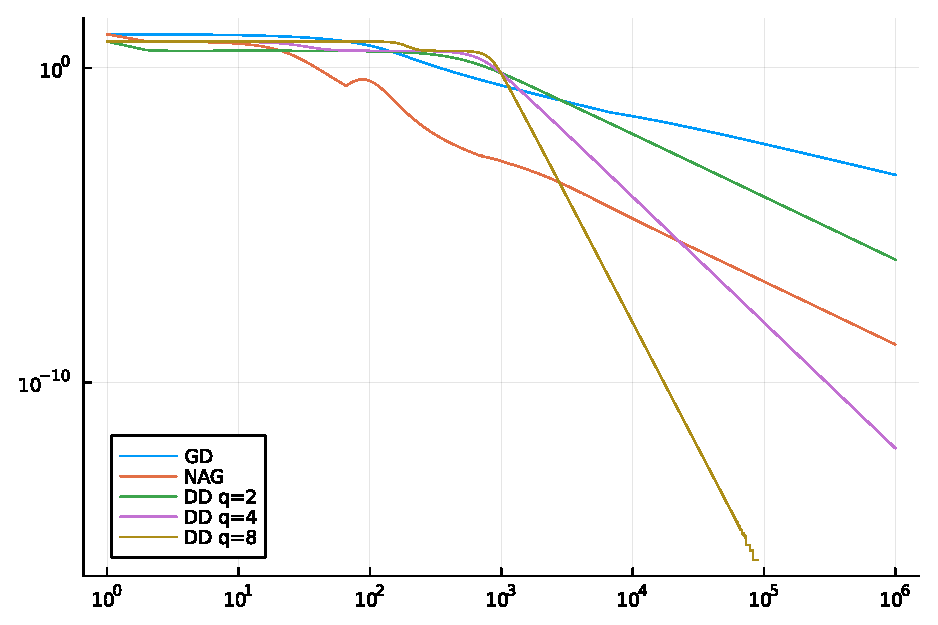
\includegraphics[width=\textwidth]{"assets/logistic.pdf"}
        \caption{}
        \label{fig:logistic}
    \end{subfigure}
    \caption{Experimental results comparing DD with GD and NAG. (a) Convergence path of GD, NAG and DD with different Runge-Kutta integrators of degree $s=1, 2, 4$ on $L_2$ loss. (b) The optimization of $L_2$ loss by DD with different choices of $q$ values with 4-th order Runge-Kutta integrator RK4. (c) Minimization of $L_4$ loss by GD, NAG and DD with different $q$ vaues with a 2-nd order Runge-Kutta integrator. (d) Minimization of logistic loss by GD, NAG and DD with different $q$ vaues with a 4-th order Runge-Kutta integrator.}
    \label{Numerical}
\end{figure}

First, we explore the optimization path of a quadratic function, the $L_2$ loss, with respecct to iteration. In particular, we labeled half of the generated data by 0 and the rest by 1. In Figure \ref{fig:l2-1}, the ODE is discretized for $p=2$ with different Runge-Kutta integrators with $s \in \{ 1,2,4 \}$ and compared against GD and NAG algorithm. We can find that except the integrator with $s=1$ can not converge due to the unstability of the differential format itself, the DD methods shows superiority over GD. By using higher order iterator, the local acceleration is achieved and 4th order DD even converges faster than NAG (although for each iteration, it is obviously more costly than NAG). In Figure \ref{fig:l2-2}, we explore the effect of $q$ is the ODE. Since in the article $p$ keeps the same as the one in Assumption \ref{assumption1}, thus we denotes $q$ the true parameter used in the ODE as below
$$
    \ddot x(t) + \frac{2q+1}{t}\dot x(t)+q^2 t^{q-2}\nabla  f(x(t)) = 0.
$$
We optimize the same $L_2$ loss with different values of $q$. By selecting smaller learning rates and increasing the numerical precision by using longer floats, the phenomenon that DD method diverges when $q>2$ is not observed. Instead, we found that for $q \in \{ 2,3,4,5 \}$, larger $q$ will give out faster convergence.

Then the minimization of $L_4$ loss (Figure \ref{l4}) and logistic loss (Figure \ref{fig:logistic}) is studied. We use 2-nd order Runge-Kutta integrator SSPRK22 for logistic loss optimization and 4-th order Runge-Kutta integrator RK4 for $L_4$ loss. As shown in Figure \ref{l4} and \ref{fig:logistic}, the loss decrease faster for larger $q$, as we can observed in above experiment about $L_2$ loss.
\section{Discussion}

\subsection{Intuitive knowledge}

Roughly speaking, this article allows for the design of optimization
methods via direct discretization using Runge-Kutta integrators. However, the two
assumptions required would be essential. \textbf{Assumption 1} quantifies the local flatness
of convex functions in a way, and it actually contradicts our normal impression that
gradient descent converges fast when the objective is not flat. This innovative discovery
may inspire people to hold a more modern opinion towards the connection between
convergence and local flatness. Also, the article claims that with careful
analysis, discretizing ODE can preserve some of its trajectories properties.
As a result, making further research on continuous ODE or appling the KR method to
more general ODE cases can be valuable.

\subsection{Potential research directions}

To make further steps, there are quite some choices to take. The article uses conditions
of higher-order differentiability to finally achieve an algorithm involving only
first-order differential. We can see if allowing second and higher-order differential in
the final algorithm will make things different, though in that case NAG method
would be useless so we have to find another acceleration method to start with. Furthermore,
as discussed above, the influence of local flatness to the convergence behaviour in
discretized integraters is worth digging. How does the process of integration approaching
actually work? What's the instinctive impact of local differentials and higher-order
differentials? With techniques we know, some new results might be discovered.\\\\
To make a bold move, adding some random part to the conditions might leads to some
interesting facts.\\\\
\textcolor{red}{If someone comes up with more technical idea or just something creative,
  we can add here.}


\printbibliography

\end{document}